\documentclass{article}

\usepackage{../arxiv}

\usepackage[utf8]{inputenc} % allow utf-8 input
\usepackage[T1]{fontenc}    % use 8-bit T1 fonts
\usepackage{hyperref}       % hyperlinks
\usepackage{url}            % simple URL typesetting
\usepackage{booktabs}       % professional-quality tables
\usepackage{amsfonts}       % blackboard math symbols
\usepackage{nicefrac}       % compact symbols for 1/2, etc.
\usepackage{microtype}      % microtypography
\usepackage{cleveref}       % smart cross-referencing
\usepackage{graphicx}
\usepackage{caption}
\usepackage{algorithm}
\usepackage{algpseudocode}
\usepackage{ragged2e}
\usepackage[style=numeric,sorting=none]{biblatex}
\usepackage[symbol]{footmisc}
\usepackage{tabu}
\usepackage{color}
\usepackage{listings}

\addbibresource{\jobname.bib}

% syntax highlighting for Rust:
% https://www.reddit.com/r/rust/comments/f7ocdx/rust_the_bookstyle_syntax_highlighting_for_latex/
\definecolor{GrayCodeBlock}{RGB}{241,241,241}
\definecolor{BlackText}{RGB}{110,107,94}
\definecolor{RedTypename}{RGB}{182,86,17}
\definecolor{GreenString}{RGB}{96,172,57}
\definecolor{PurpleKeyword}{RGB}{184,84,212}
\definecolor{GrayComment}{RGB}{170,170,170}
\definecolor{GoldDocumentation}{RGB}{180,165,45}
\lstdefinelanguage{rust}
{
    columns=fullflexible,
    keepspaces=true,
    frame=single,
    framesep=0pt,
    framerule=0pt,
    framexleftmargin=12pt,
    framexrightmargin=12pt,
    framextopmargin=12pt,
    framexbottommargin=0pt,
    xleftmargin=12pt,
    xrightmargin=12pt,
    backgroundcolor=\color{GrayCodeBlock},
    basicstyle=\ttfamily\color{BlackText},
    keywords={
        true,false,
        unsafe,async,await,move,
        use,pub,crate,super,self,mod,
        struct,enum,fn,const,static,let,mut,ref,type,impl,dyn,trait,where,as,
        break,continue,if,else,while,for,loop,match,return,yield,in
    },
    keywordstyle=\color{PurpleKeyword},
    ndkeywords={
        bool,u8,u16,u32,u64,u128,i8,i16,i32,i64,i128,char,str,
        Self,Option,Some,None,Result,Ok,Err,String,Box,Vec,Rc,Arc,Cell,RefCell,HashMap,BTreeMap,
        macro_rules
    },
    ndkeywordstyle=\color{RedTypename},
    comment=[l][\color{GrayComment}\slshape]{//},
    morecomment=[s][\color{GrayComment}\slshape]{/*}{*/},
    morecomment=[l][\color{GoldDocumentation}\slshape]{///},
    morecomment=[s][\color{GoldDocumentation}\slshape]{/*!}{*/},
    morecomment=[l][\color{GoldDocumentation}\slshape]{//!},
    morecomment=[s][\color{RedTypename}]{\#![}{]},
    morecomment=[s][\color{RedTypename}]{\#[}{]},
    stringstyle=\color{GreenString},
    string=[b]"
}

\title{Dango DEX}

\author{
  Larry Engineer \\
	Left Curve Software \\
	\texttt{larry@leftcurve.io} \\
}

\date{Initial version: UNRELEASED}

\begin{document}
\maketitle

\begin{abstract}
  Dango DEX is an onchain limit order book exchange that tackles three main challenges faced by today's DEXs: the inaccessibility of order book market making to retail investors due to the high level of sophistication required; reduced yield for AMM LPs due to arbitrage flow; and malicious MEV. Dango DEX enshrines its order book with a passive liquidity pool that actively adjusts its quotes utilizing a low latency oracle, and clears orders using frequent, uniform price, sealed bid auctions. Overall, Dango DEX seeks to democratize market making on order books, minimize toxic arbitrage flow, while maximize organic, non-arbitrage flow.
\end{abstract}

Dango DEX is one of the two flagship apps of our upcoming DeFi ecosystem, Dango,\supercite{dangotwitter} besides the cross-collateralized \textbf{credit account}. To learn more about the credit account, see \cite{creditaccountmarsforum,creditaccountbuidlkeynote}.

This paper is laid out as follows: 1) identifying the problems in today's DeFi exchanges; 2) analyzing the causes of the problems; and 3) proposing our solutions.

\section{Background}

\subsection{TradFi}

In traditional finance (TradFi) markets, \textbf{limit order book} (LOB) is the primary venue for trading. A limit order consists of the quantity of asset the trader wishes to buy or sell, and a limit price at which or better the trade must be executed.

\textbf{Market makers} (MMs) facilitate trades by strategically placing orders below and above the prevailing market price. E.g., suppose Apple stock (AAPL) is trading at \$200. An MM may place a BUY order at \$199.5 and a SELL order at \$200.5. The \$1 difference is known as the \textbf{spread}. If a trader sells AAPL to the MM by taking the said BUY order, then another trader buys AAPL by taking the said SELL order, the MM has made \$1. This is typically described as the MM ``making money on the spread''.

MMs bet the stock's price goes side ways, i.e. there is roughly the same buy and sell volume. If the market only goes one way, the MM accumulates one side of the inventory, which is the underperforming side. E.g., if there is consistently more sellers of AAPL than buyers, the MM's BUY orders get consistently picked up more often than his SELL orders do, he would accumuate a large inventory of AAPL, an asset that's going down in price. He would underperform the trading strategy that simply holds the initial inventory without market making. This is known as the \textbf{inventory risk} which is rooted in the asset's price volatility. MMs usually use \textbf{hedging} to mitigate this risk.

Another major risk faced by MMs comes from \textbf{information asymmetry}. Suppose Apple releases a better-than-expected earnings report, causing the ``fair value'' of its stock to jump to \$300. However, the MM is still placing orders around the \textbf{stale price} of \$200, either because he isn't aware of the news or is slow to update the quotes. An \textbf{informed trader} or \textbf{high frequency trader} (HFT) is one who is well informed on the news and is able to execute trades faster. The NFT is able to pick up the MM's SELL order at \$200.5 and immediately resell the stock for \$300, pocketing the arbitrage gain. The MM loses value because he has sold the stock at a much lower-than-market price. Both MMs and HFTs invest significant amount of resources to improve their execution speed in an ``arms race''.\supercite{frequentbatchauctions} This is a very high level of sophistication that makes market making inaccessible to most retail investors.

\subsection{DeFi}

Maintaining a LOB and executing orders is computationally costly. For this reason, onchain finance has historically relied on \textbf{constant function market makers} (CFMMs) instead of LOBs. (That is, until the recent advent of high performance blockchains such as Solana, Diem, Dydx, and Hyperliquid.)

A CFMM, instead of maintaining a book of limit orders, maintains a pool of liquidity and quotes prices based on a predefined \textbf{invariant}. An invariant is a function $f(x, y)$ that yields the same value before and after a trade, where $x$ and $y$ are the quantities of the \textbf{base asset} and the \textbf{quote asset}, respectively (known as the pool's \textbf{reserves}):

\begin{equation}
  f(x, y) = K \ (\mathrm{constant})
\end{equation}

Suppose a pool contains base asset $\mathtt{A}$ and quote asset $\mathtt{B}$ of reserves $A$ and $B$, respectively, and a trader wishes to swap $a$ amount of $\mathtt{A}$ into $\mathtt{B}$. The pool would determine the output amount $b$ by solving the equation:

\begin{equation}
  f(A, B) = f(A + a, B - b) = K
\end{equation}

Similarly, a swap from $b$ amount of $\mathtt{B}$ into $\mathtt{A}$ will have its output amount $a$ determined by:

\begin{equation}
  f(A, B) = f(A - a, B + b) = K
\end{equation}

Note that this doesn't consider trading fees. Since there is no such thing as ``spread'' in CFMMs as in LOBs, the pool makes money for its \textbf{liquidity providers} (LPs) by charging a fee on each trade. Specifically, a small portion of the trade's output is deducted and injected into the pool. The value of $K$ slightly increases as a result. As such, $K$ can be considered as a measurement of how much liquidity there is in the pool, regardless of the asset prices.

CFMMs share the same types of risks as LOBs, but to different degrees. Firstly, LPs in an CFMM pool bet the two assets' relative price stays roughly constant. If one asset's price drops relative to the other, the pool accumulates this underperforming asset. Not considering fees, this would underperform the strategy of simply holding the two assets and not market making. This is known as \textbf{impermanent loss} (IL). IL is essentially the same thing as inventory risk for LOBs, caused by the asset's volatility, and can be mitigated through hedging.

In terms of information asymmetry, however,  CFMMs are categorically worse than LOBs. A traditional CFMM \textit{never} adjusts its quotes in response to new information. Therefore, from an LP's perspective, a CFMM always trades at worse-than-market prices. The loss incurred from this is known as \textbf{loss-versus-rebalancing} (LVR).\supercite{lvr}

A \textbf{searcher} is a trader who scans onchain DEXs for stale prices, and executes CEX-DEX arbitrage. Since arbitraging is highly competitive, searchers share portions of their arbitrage gains with the chain's block builders by paying ``tips''.

There are other ways besides arbitrage with which searchers make money. Once of these is \textbf{sandwich attacks}, where a searcher bribes the block builders to insert transactions (txns) immediately before and after a user's trade. These txns manipulate prices in the DEX, give the user a worse execution price, while profiting the trader. Sandwich attack is not inheritly a problem of CFMMs; onchain LOBs can be similarly attacked. Instead, it's a result of the fact that user orders are broadcasted transparently through the network. In comparison, user orders in CEXs are kept private unless filled.

\subsection{The problems}

Through the above discussions, we have identified three problems with TradFi and DeFi exchanges:

\begin{enumerate}
  \item Market making in LOBs is not accessible to retail investors because of the high level of sophistication required, which is in larger part a result of the HFT arms race.
  \item CFMM democratizes market making to retail investors, but they generally don't make money or even lose money because of LVR.
  \item Traders are susceptible to sandwich attacks due to the lack of privacy.
\end{enumerate}

We do not aim to solve IL / inventory risk, because it's rooted in the assets' volalitity, not a problem with DEX design. We can imagine vaults that automatically deploy hedging strategies to mitigate it.

\section{Our solution}

We propose solving the above problems as follows:

\begin{itemize}
  \item Create a LOB that has an enshrined passive liquidity pool. The pool will place orders in the LOB following a CFMM invariant.
  \item In order to mitigate LVR, we:
        \begin{itemize}
          \item make available a high-frequency, low-latency oracle reporting the latest prevailing market prices;
          \item incorporate this oracle feed into the liquidity pool's CFMM invariant;
          \item give the pool priority in adjusting its quotes over other traders.
        \end{itemize}
  \item In order to mitigate MEV, we:
        \begin{itemize}
          \item use a private mempool so that user orders aren't public;
          \item use frequent, uniform price, sealed-bid auctions to match and execute orders, so that HFTs don't have time advantage over other traders.
        \end{itemize}
\end{itemize}

First, let's discuss how to incorporate a passive CFMM pool into a LOB. Let's start with the simplest form of CFMM invariants, the \textbf{xyk invariant}.

\subsection{Passive liquidity on a LOB following the xyk invariant}

The xyk invariant, proposed by Martin Köppelmann,\supercite{xykamm} has the form:

\begin{equation}
  f(x, y) = x \cdot y = K
\end{equation}

How would the pool place orders in a LOB, following this invariant? Let's start with the BUY side. Suppose the pool has reserves $x = A$ and $y = B$. It places a BUY order, offering $b_{\mathrm{bid}}$ units of the quote asset $\mathtt{B}$ in exchange for $a_{\mathrm{bid}}$ units of the base asset $\mathtt{A}$, at price $p$. The invariant must hold:

\begin{equation}
  A B = (A + a_{\mathrm{bid}}) (B - b_{\mathrm{bid}})
\end{equation}

By definition:

\begin{equation}
  p = \frac{b_{\mathrm{bid}}}{a_{\mathrm{bid}}}
\end{equation}

Putting these together, we can easily solve:

\begin{equation}
  a_{\mathrm{bid}} = -A + \frac{B}{p}
\end{equation}

Similarly, on the SELL side, we have:

\begin{equation}
  A B = (A - a_{\mathrm{ask}}) (B + b_{\mathrm{ask}})
\end{equation}

\begin{equation}
  p = \frac{b_{\mathrm{ask}}}{a_{\mathrm{ask}}}
\end{equation}

\begin{equation}
  a_{\mathrm{ask}} = A - \frac{B}{p}
\end{equation}

It's immediately obvious that in both cases, if $p = \frac{B}{A}$, then $a = 0$. This is a special price, at which the pool does not offer to buy or sell in any amount, we denote as the \textbf{pool price} $p_{\mathrm{pool}}$. In the most general case, $p_{\mathrm{pool}}$ is \textit{the price at which the trade swapping an infinitesimal amount of base asset into the quote asset is executed}:

\begin{equation}
  p_{\mathrm{pool}}(x, y) = - \frac{\mathrm{d}y}{\mathrm{d}x}
\end{equation}

Since $x$ and $y$ follows $f(x, y) = K$, using the chain rule of multivariant functions, we can get:

\begin{equation}
  p_{\mathrm{pool}}(x, y) = \frac{\frac{\partial f}{\partial x}}{\frac{\partial f}{\partial y}}
\end{equation}

For the xyk invariant specifically, this is:

\begin{equation}
  p_{\mathrm{pool}}(x, y) = \frac{y}{x}
\end{equation}

Intuitively, $p_{\mathrm{pool}}$ is the ``inherit'' price mplied by its reserves. The pool will place orders around this price.

At any price $p < p_{\mathrm{pool}}$, $a_{\mathrm{bid}} > 0$. This can be understood as the pool offering to buy $a_{\mathrm{bid}}$ amount of the base asset between prices $p$ and $p_{\mathrm{pool}}$.

Of course, prices LOBs are discret, separated by \textbf{ticks}. Let's say the tick size is $\Delta p$. Consider the price one tick above $p$, $p' = p + \Delta p$:

\begin{equation}
  a'_{\mathrm{bid}} = -A + \frac{B}{p'}
\end{equation}

\begin{equation}
  \Delta a_{\mathrm{bid}} = a_{\mathrm{bid}} - a'_{\mathrm{bid}} = B \left(\frac{1}{p} - \frac{1}{p'} \right) = B \frac{\Delta p}{p (p + \Delta p)}
\end{equation}

This is the quantity of BUY order that the pool will place at price $p$.

Similarly, one the SELL side, for two prices $p' = p - \Delta p$ and $p' > p_{\mathrm{pool}}$:

\begin{equation}
  \Delta a_{\mathrm{ask}} = a_{\mathrm{ask}} - a'_{\mathrm{ask}} = B \left(\frac{1}{p} - \frac{1}{p'} \right) = B \frac{\Delta p}{p (p - \Delta p)}
\end{equation}

\subsubsection{Example}

Consider a pool containing base asset SOL of quantity $A = 1$ and quote asset USD of quantity $B = 200$. Pool price $p_{\mathrm{pool}} = 200$. \hyperref[fig:1]{Figure 1} plots the order sizes $\Delta a_{\mathrm{bid}}$, $\Delta a_{\mathrm{ask}}$ as well as cumulative BUY/SELL demand agianst price $p$.

\begin{figure}
  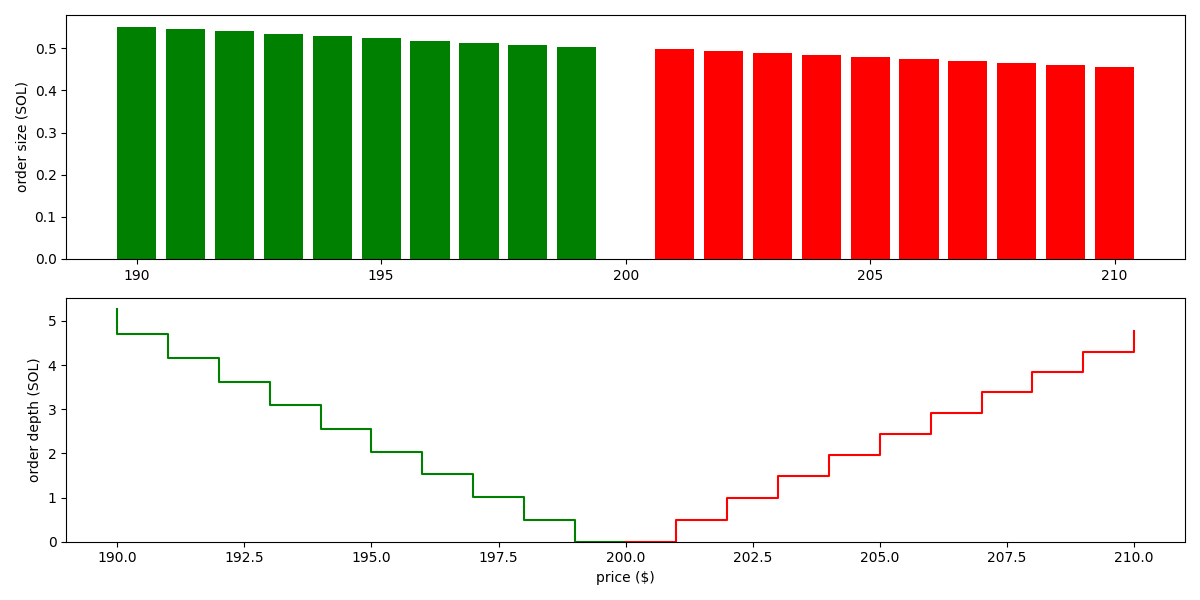
\includegraphics[width=\textwidth]{1-xyk.png}
  \caption{Order size and depth following the xyk invariant}
  \label{fig:1}
\end{figure}

\subsubsection{Bried summary so far}

We have established the concept of pool price $p_{\mathrm{pool}}$, and a way to derive BUY/SELL order size $\Delta a_{\mathrm{bid}}$ and $\Delta a_{\mathrm{ask}}$ in relation to a given price $p$.

Looking at the order depth chart of the xyk invariant, it puts liquidity roughly evenly over a wide range of prices. This in capital inefficient; ideally, we want to concentrate the liquidity in the region close to $p_{\mathrm{pool}}$.

Additionally, this invariant is susceptible to LVR, as $p_{\mathrm{pool}}$ does not adjust in response to the change of price in CEXs.

\subsection{Passive liquidity on a LOB following the Solidly invariant}

The Solidly invariant, conceived by Andre Cronje\supercite{andrecronjetwitter} and popularized by Velodrome\supercite{velodrome} and its forks,\supercite{aerodrome} has the form:

\begin{equation}
  f(x, y) = x^3 y + x y^3 = K
\end{equation}

This formula assumes the two assets have the same price. In case they're not the same price, and we have an oracle feed indicating that one unit of $x$ is equivalent in value to $R$ units of $y$, the formula can be updated to:

\begin{equation}
  f(x, y) = x^3 \left( \frac{y}{R} \right) + x \left( \frac{y}{R} \right)^3
\end{equation}

The pool price is:

\begin{equation}
  p_{\mathrm{pool}}(x, y) = \frac{3 R^2 x^2 y + y^3}{R^2 x^3 + 3 R x y^2}
\end{equation}

Let's derive $a_{\mathrm{bid}}$ the same way as we did for the xyk pool. Suppose the pool as reserves $A$ and $B$ prior to the swap:

\begin{equation}
  f(A, B) = A^3 \left( \frac{B}{R} \right) + A \left( \frac{B}{R} \right)^3 = K
\end{equation}

On the BUY side, a trader inputs $a_{\mathrm{bid}}$ units of base asset, receives $b_{\mathrm{bid}}$ units of quote asset. The trade executes at the price:

\begin{equation}
  p = \frac{b_{\mathrm{bid}}}{a_{\mathrm{bid}}}
\end{equation}

For convenience, let's denote:

\begin{equation}
  \alpha = A + a_{\mathrm{bid}}
\end{equation}

\begin{equation}
  \beta = \frac{B - b_{\mathrm{bid}}}{R} = \frac{B - p a_{\mathrm{bid}}}{R}
\end{equation}

Essentially, $\alpha$ is the pool's base asset reserve after the trade, $\beta$ is the quote asset reserve after the trade, adjusted for the oracle price.

The invariant must also hold after the trade:

\begin{equation}
  f(A + a_{\mathrm{bid}}, B - b_{\mathrm{bid}}) = \alpha^3 \beta + \alpha \beta^3 = K
\end{equation}

This is a 4th-degree (quartic) equation, so finding a closed form solution is not feasible. Instead, we solve it by \textbf{Newton's method}. Define:

\begin{equation}
  g(a_{\mathrm{bid}}) = \alpha^3 \beta + \alpha \beta^3 - K
\end{equation}

We must solve for $a_{\mathrm{bid}}$ such that $g(a_{\mathrm{bid}}) = 0$. This can be done by:

\begin{algorithm}
  \caption{Newton's method for solving $g(a_{\mathrm{bid}}) = 0$}
  \begin{algorithmic}
    \State $a_0 \gets A$
    \For{$n = 1, 2, 3, \dots$}
    \State $a_n \gets a_{n-1} - \frac{g(a_{n-1})}{g'(a_{n-1})}$
    \If{converge}
    \State return $a_n$ as the solution for $a_{\mathrm{bid}}$
    \EndIf
    \EndFor
  \end{algorithmic}
\end{algorithm}

where

\begin{equation}
  g'(a_{\mathrm{bid}}) = -\frac{p}{R} \alpha^3 + a \alpha^2 \beta - \frac{3p}{R} \alpha \beta^2 + \beta^3
\end{equation}

The choice of the initial value $a_0$ is important. This is because $g(a_{\mathrm{bid}}) = 0$ has a trivial solution of $a_{\mathrm{bid}} = 0$, which corresponding to not placing an order at all. Instead, we want to find the non-trivial solution of $a_{\mathrm{bid}} > 0$. Emprically, choosing $a_0 = A$ always gives us the intended solution.

For the SELL side, we do exactly the same, except for:

\begin{equation}
  \alpha = A - a_{\mathrm{ask}}
\end{equation}

\begin{equation}
  \beta = \frac{B + b_{\mathrm{ask}}}{R} = \frac{B + p a_{\mathrm{ask}}}{R}
\end{equation}

\begin{equation}
  g'(a_{\mathrm{ask}}) = \frac{p}{R} \alpha^3 - a \alpha^2 \beta + \frac{3p}{R} \alpha \beta^2 - \beta^3
\end{equation}

\subsubsection{Example}

Following the same example of SOL-USD pool in the previous discussions, assuming oracle price $R = 200$ (USD per SOL), the liquidity depth can be computed and plotted in \hyperref[fig:2]{Figure 2}.

\begin{figure}
  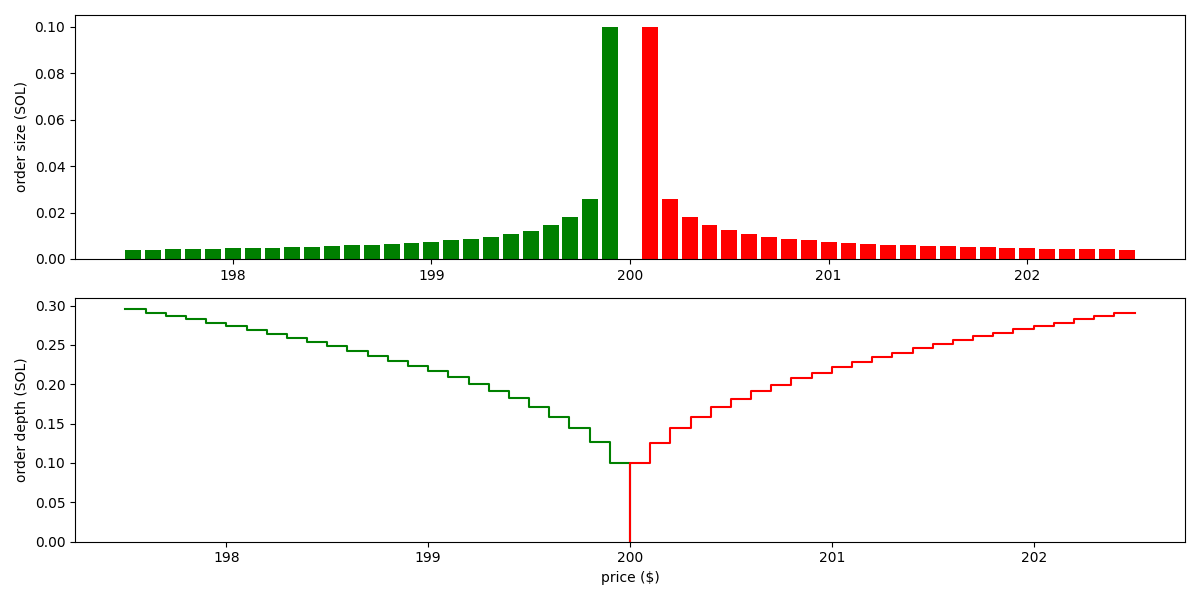
\includegraphics[width=\textwidth]{2-solidly.png}
  \caption{Order size and depth following the Solidly invariant}
  \label{fig:2}
\end{figure}

It's obvious that liquidity is now indeed concentrated around the pool price.

In general, however, $R$ does not match exactly the composition of assets in the pool. In order to mitigate LVR, we need $p_{\mathrm{pool}}$ to closely track $R$. \hyperref[fig:3]{Figure 3} plots the deviation of $p_{\mathrm{pool}}$ from $R$ against $R$.

\begin{figure}
  \centering
  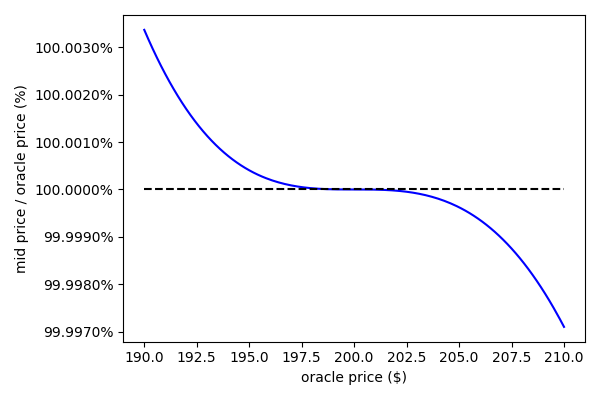
\includegraphics[width=4in]{3-solidly-pool-price-vs-oracle.png}
  \caption{Deviation of pool price from oracle price}
  \label{fig:3}
\end{figure}

As seen, the deviation does not exceed 0.003\% when oracle price jumps less than \textasciitilde 5\%. As such, we believe the pool is not ssusceptible to LVR, given that the oracle price's latency is sufficient low to reflect the true asset price.

\subsection{Minimizing LVR with oracle-imformed CFMM}

In order for the passive liquidity pool to provide accurate quotes, it's important that:

\begin{itemize}
  \item it has access to a low-latency oracle that accurately reports the up-to-date market prices; and,
  \item it must be able to adjust its orders before any other trader is able to pick up the scale quotes.
\end{itemize}

For the oracle, we propose using Pyth Laser,\supercite{pythlaser} which provides ultra fast price feeds with 1 millisecond updates. Each block, the proposer fetches the prices and submit them onchain in a transaction on the very top of the block.

To ensure the passive liquidity pool has priority in updating quotes, we utilize a technique which we dub \textbf{virtual order book}. Instead of physically placing orders, the pool constructs a virtual order book, based on its asset reserves and oracle price, prior to any order being matched. The matching engine then combines the real, physical order book with the virtual book before performing matching. See \hyperref[sec:appendixa]{Appendix A} for code snippets demonstrating this idea.

\subsection{Mitigating MEV with frequent batch auctions}

A searcher relies on two prerequisites both being satisfied in order to pull off malicious MEV activities:

\begin{itemize}
  \item user orders are broadcasted transparently, unencrypted, through the public p2p network;
  \item trades are possibly executed at different prices throughout the same block.
\end{itemize}

On the first point, we believe the endgame solution is encrypted mempool.\supercite{encryptedmempool} However, to achieve a faster go-to-market, we propose a faster interim solution: the Dango blockchain to run on a proof-of-authority validator set; validators to configure their mempools such that they only receive transactions, and broadcast only to other validators, but not to any other node. Users will broadcast their transactions directly to the validators. As such, assume validators themselves do not engage in malicious MEV (as they will be contractually obliged to), user transactions can be considered private.

On the second point, we propose to execute orders using the frequent batch auctions (FBAs) approach.\supercite{frequentbatchauctions,frequentbatchauctions2} Specifically, the flow of a block would be:

\begin{enumerate}
  \item In the first transaction, the proposer submits up-to-date oracle prices.
  \item Users submit orders. These orders are stored in a \textbf{transient storage} in the DEX smart contract. Data in the transient storage only persists through one block (wiped at the end of the block) and importantly, cannot be queried by other contracts.
  \item After all user transactions have been processed, the DEX contract iterates through all trading pairs that have received new orders in this block and attempts to match the orders:
        \begin{enumerate}
          \item Add new orders in the transient storage into the order book.
          \item Compute the virtual order book of the passive liquidity pool, based on the pool's asset reserves and oracle price.
          \item Combine the two books in (a) and (b) and perform order matching through a uniform price auction.\supercite{uniformpriceauctions} The objective is to find the intersection between the cumulative supply and demand curves, which is the price that maximizes trading volume.
          \item Given the clearing price found in (c), fill the orders, send the output funds to traders.
        \end{enumerate}
\end{enumerate}

There are two notable elements in this:

\begin{itemize}
  \item This is a \textbf{sealed-bid} auction. Given that users broadcast transactions to a private mempool, and orders are stored in the transient storage, the orders are kept confidential prior to the auction.
  \item This is a \textbf{uniform price} auction. All trades are settled at the same clearing price, so it's literally impossible to execute sandwich attacks.
\end{itemize}

\section{Conclusion}

We have identified and analyzed the causes of three main problem faced by today's DEXs. We propose Dango DEX as a solution. See \hyperref[tab:conclusion]{Table 1} for a summary.

\begin{table}
  \tabulinesep=2.5mm
  \newcolumntype{Y}{>{\RaggedRight}X} % avoid hyphenation when wrapping words in tabularx
  \begin{tabu} to \textwidth {YYY}
    \toprule
    \textbf{The problem}                                                                                       & \textbf{The cause} & \textbf{Our solution} \\
    \midrule
    Market making on LOBs is not accessible for retail investors                                               &
    High level of sophistication is required                                                                   &
    Our LOB to be enshrined with a passive liquidity pool that follows the Solidly AMM curve                                                                \\
    \hline
    LVR                                                                                                        &
    CFMMs do not actively adjust quotes in reaction to changes in asset prices                                 &
    Our passive liquidity pool to adjust its curve based on a low-latency oracle feed, with priority over any other trader                                  \\
    \hline
    MEV                                                                                                        &
    User orders are broadcasted publicly, and are settled at potentially different prices throughout the block &
    Private mempool; frequent sealed-bid batch auctions at uniform prices                                                                                   \\
    \bottomrule
  \end{tabu}
  \vspace*{0.1in}
  \caption{Conclusion}
  \label{tab:conclusion}
\end{table}

\appendix
\section{Suggested implementation}
\label{sec:appendixa}

We suggest performing FBA at the frequency of once per block. Research suggests the optimal frequency for FBA is 0.2--0.9 second;\supercite{optimalspeed} we suggest picking a block time within this range.

The specific algorithm for matching the orders is described below, in Rust pseudocode.

First, we define the following types:

\begin{minipage}{\linewidth}
  \begin{lstlisting}[language=rust]
enum Direction {
    Bid,
    Ask,
}

struct Order {
    /// The order's limit price.
    pub price: Decimal,
    /// The quantity of that's not yet filled, measured in the base asset.
    pub quantity: Uint128,
}
  \end{lstlisting}
\end{minipage}

Second, the DEX contract must be capable of iterating over orders in the book following the \textbf{price-time priority}. That is, orders with better prices (for BUY orders, the higher; for SELL orders, the lower) come first; for orders with the same price, the older ones come first. We abstract this as a Rust iterator type:

\begin{minipage}{\linewidth}
  \vspace*{0.1in}
  \begin{lstlisting}[language=rust]
type OrderIterator<'a> = Box<dyn Iterator<Item = Order> + 'a>;
  \end{lstlisting}
\end{minipage}

Third, the passive liquidity pool must implement the following trait:

\begin{minipage}{\linewidth}
  \vspace*{0.1in}
  \begin{lstlisting}[language=rust]
trait LiquidityPool {
    /// Return an iterator over the BUY orders that the passive liquidity pool
    /// would place in the order book following its CFMM invariant, given the
    /// latest oracle price.
    fn get_bids<'a>(&'a self, oracle_price: Decimal) -> OrderIterator<'a>;

    /// Similarly, return an iterator over SELL orders.
    fn get_asks<'a>(&'a self, oracle_price: Decimal) -> OrderIterator<'a>;
}
  \end{lstlisting}
\end{minipage}

When matching orders, we work with two order books: a ``\textbf{physical}'' book that contains orders submitted by users, and a ``\textbf{virtual}'' book that contains orders that the passive liquidity pool would place.

We must match orders from the two books at the same time. For this we can use a the following merged iterator:

\begin{minipage}{\linewidth}
  \vspace*{0.1in}
  \begin{lstlisting}[language=rust]
struct MergedIterator {
    a: Peekable<Item = Order>,
    b: Peekable<Item = Order>,
    direction: Direction,
}

impl MergedIterator {
    pub fn new<A, B>(a: A, b: B) -> Self
    where
        A: Iterator<Item = Order>,
        B: Iterator<Item = Order>,
    {
        Self {
            a: a.peekable(),
            b: b.peekable(),
        }
    }
}

impl Iterator<Item = Order> for MergedIterator {
    fn next(&mut self) -> Option<Order> {
        match (self.a.peek(), self.b.peek()) => {
            // Both iterators have orders left. Return the one with the better
            // price. If prices are the same, we arbitrarily choose the order in B.
            (Some(a), Some(b)) => {
                match self.direction {
                    Direction::Bid if a.price > b.price
                    | Direction::Ask if a.price < b.price => a.next(),
                    _ => b.next(),
                }
            },
            // A still has orders, but B has run out. Return the next order in A.
            (Some(_a), None) => a.next(),
            // B still has orders, but A has run out. Return the next order in B.
            (None, Some(_b)) => a.next(),
            // Both iterators have run out of orders. We're done.
            (None, None) => None,
        }
    }
}
  \end{lstlisting}
\end{minipage}

The DEX smart contract prepares iterators over orders in the two books, and combine them using \texttt{MergedIterator}:

\begin{minipage}{\linewidth}
  \vspace*{0.1in}
  \begin{lstlisting}[language=rust]
let physical_bid_iter: OrderIterator = /* ... */;
let physical_ask_iter: OrderIterator = /* ... */;

let virtual_bid_iter: OrderIterator = /* ... */;
let virtual_bid_iter: OrderIterator = /* ... */;

// Use the virtual book iterators as the B in MergedIterator, such that
// orders from the passive liquidity pool is prioritized.
let bid_iter = MergedIterator::new(physical_bid_iter, physical_ask_iter);
let ask_iter = MergedIterator::new(virtual_bid_iter, virtual_bid_iter);
  \end{lstlisting}
\end{minipage}

Note that we compute the virtual orders based on the latest oracle price \textit{before orders are matched}. This ensures the passively liquidity pool always quotes the latest price, providing its LVR resistance.

Then, we use the following pure function to find the clearing price:

\begin{minipage}{\linewidth}
  \vspace*{0.1in}
  \begin{lstlisting}[language=rust]
struct MatchingOutcome {
    /// The range of prices that results in the maximal volume.
    /// The clearing price can be chosen as any value within this range.
    /// It's up to the caller to make the choice.
    range: Option<(Decimal, Decimal)>,
    /// The maximal volume.
    volume: Uint128,
    /// List of BUY orders that have found a match.
    bids: Vec<Order>,
    /// List of SELL orders that have found a match.
    asks: Vec<Order>,
}

fn clear_orders(
    mut bid_iter: OrderIterator,
    mut ask_iter: OrderIterator,
) -> MatchingOutcome {
    let mut maybe_bid = bids.next();
    let mut bids = Vec::new();
    let mut bid_is_new = true;
    let mut bid_volume = Uint128::ZERO;
    let mut maybe_ask = asks.next();
    let mut asks = Vec::new();
    let mut ask_is_new = true;
    let mut ask_volume = Uint128::ZERO;
    let mut range = None;

    loop {
        // If we run out of orders on either side, then we're done.
        let (Some(bid), Some(ask)) = (maybe_bid, maybe_ask) else {
            break;
        }

        // If the prices don't cross, then we're done.
        if bid.price < ask.price {
            break;
        }

        range = Some((ask.price, bid.price));

        if bid_is_new {
            bids.push(bid);
            bid_volume += bid.quantity;
        }

        if ask_is_new {
            asks.push(ask);
            ask_volume += ask.quantity;
        }

        if bid_volume <= ask_volume {
            bid = bid_iter.next();
  \end{lstlisting}
\end{minipage}

\begin{minipage}{\linewidth}
  \vspace*{0.1in}
  \begin{lstlisting}[language=rust]
            bid_is_new = true;
        } else {
            bid_is_new = false;
        }

        if ask_volume <= bid_volume {
            ask = ask_iter.next();
            ask_is_new = true;
        } else {
            ask_is_new = false;
        }
    }

    let volume = bid_volume.min(ask_volume);

    MatchingOutcome { range, volume, bids, asks }
}
  \end{lstlisting}
\end{minipage}

Once we have the clearing price, clearing the orders is trivial (which involves updating the order state in the book and refund assets to traders) so we don't discuss them here.

\subsection{Customizations}

In the above formulation of the passive liquidity pool, the pool places orders every tick, starting one tick above and below $p_{\mathrm{pool}}$. This can be customized by introducing two additional parameters:

\begin{itemize}
  \item \textbf{Cadence}: The pool can instead place an order every $N$ ticks. Alternatively, it can place orders more densely when close to $p_{\mathrm{pool}}$, but more loosely when farther away. Either way, there will be fewer orders overall, reducing computational cost.
  \item \textbf{Spread}: The pool can place orders a few ticks further away from $p_{\mathrm{pool}}$. A bigger spread may improve the pool's profitability.The spread can either be defined as constant values, or calculated dynamically based on marketing conditions, following models such as the one proposed by Avellaneda and Stoikov.\supercite{avellanedastoikov}
\end{itemize}

\subsection{Dango's custom smart contract VM}

We recognize the above is challenging to implement in legacy virtual machines (VMs) such as the Ethereum virtual machine (EVM), due to:

\begin{itemize}
  \item In EVM, smart contract actions need to be triggered via transactions. This means each block must have a txn at the very beginning of the block to update the oracle price, and another one at the end of the block to trigger order matching. During periods of high traffic, it can be difficult to get txns into the block, not to mention ensuring they are located at the beginning and end of the block. The only way to achieve this is to utilize a centralized block builder, which introduced additional trust assumptions.\\ \\ Dango's custom smart contract VM, Grug,\supercite{grug} allows validators to submit oracle updates via Tendermint's ABCI++ API, at the top of every block. Additionally, it automatically triggers order matching via end-of-block cronjobs.\\
  \item EVM does not support iterating keys in its \texttt{mapping} data structures. This is because in EVM, the state of each contract is a hash map. Since the map keys are hashed, they are essentially randomized and thus cannot be iterated.\\ \\ In Grug, contract states are B-tree maps which support iteration.
\end{itemize}

\printbibliography

\end{document}
